% Derived from the TeX Live PGF automata manual's every-initial-by-arrow example.
\documentclass[border=2pt]{standalone}
\usepackage{tikz}
\usetikzlibrary{automata,arrows.meta}

\begin{document}
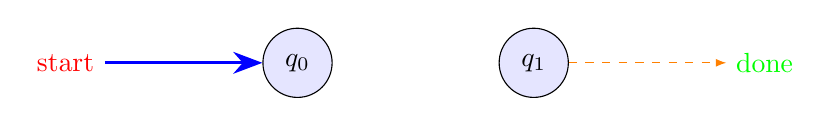
\begin{tikzpicture}[
  every initial by arrow/.style={text=red,draw=blue,very thick,-{Stealth[scale=1.25]}},
  every accepting by arrow/.style={text=green,draw=orange,dashed,-{Latex[scale=.8]}},
  every state/.style={draw=black,fill=blue!10}
]
  \node[state,initial,initial distance=2cm] (q0) at (0,0) {$q_0$};
  \node[state,accepting right,accepting distance=2cm,accepting text=done] (q1) at (3,0) {$q_1$};
\end{tikzpicture}
\end{document}
